\documentclass[12pt,letterpaper]{article}
\usepackage[secthm,mdthm,simplethm]{beel}
\usepackage[utf8]{inputenc}
\usepackage{graphicx, tcolorbox}
\usepackage[margin = 1in, top = 0.8in,bottom = 0.8in]{geometry}
\usepackage{amsmath,amsfonts,amsthm,amssymb}
\usepackage{array,comment,enumitem}
\usepackage{mathtools,thmtools}
\usepackage{multicol,tabto,setspace}
\usepackage{tikz,pgfplots,tikz-cd,venndiagram,forest}
\usepackage[all]{xy}
\usepackage{listings,fancyhdr}
\usepackage{pst-plot}
\pagestyle{fancy}

\headheight = 15 pt
\lhead{Bill Li}
\rhead{Partial Differential Equation}
\cfoot{\thepage}
\pgfplotsset{compat = 1.15}
\usetikzlibrary{fadings}

\hbadness = 10000
\tolerance = 10000

\renewcommand{\qedsymbol}{$\blacksquare$}
\renewcommand{\bar}{\overline}
\renewcommand{\b}{\mathbb}
\renewcommand{\c}{\mathcal}
\newcommand{\s}{\mathscr}

\begin{document}
\thispagestyle{empty}
$ $
\vfill
\begin{center}

\centerline{\huge \textbf{Math 126, Fall 2019}}
\centerline{\Large \textbf{Introduction to Partial Differential Equation}} 
\centerline{ Tim Laux, 3106 Etcheverry, 9-10AM}
\end{center}
\vfill
$ $
\newpage
\thispagestyle{empty}
\tableofcontents
\newpage
\setcounter{page}{1}
%!TEX root = ./main.tex
\section*{Logistics}
\begin{question}
	Why study PDE?
\end{question}
\begin{answer}
	TL;DR. It's useful.
\end{answer}
\begin{note}
	Office hour : MWF 9-10AM 895 Evans, GSI Office hour : MW 1-3 PM 1049 Evans
\end{note}
\section{where PDEs Come From}
\subsection{What is a partial differential equation?}
\begin{example}
	This is an example of ODE:
	\[ u  = u(x), \qquad \frac{d}{dx} u = u.\]
\end{example}
\begin{example}
	A PDE consist of the form
	\[ u = u(x_1, x_2, \ldots, x_d), \qquad u_{x_k} = \frac{\partial u}{\partial x_k}\]
	Where $x_i$ are scalars.
\end{example}
\begin{example}
	The most general form of a PDE of first order in two dimension, say $u = u(x,y)$ and of the form
	\[ F(x,y,u(x,y), u_x(x,y),u_y(x,y)) = 0 , \quad \mathrm{ or } \quad F(x,y,u, u_x, u_y) = 0\]

\end{example}
\begin{example}
	The most general form of a PDE of second order in two dimension, say $u = u(x,y)$ and of the form
	\[ G(x,y,u, u_x, u_y, u_{xx}, u_{yy}, u_{xy}) = 0 \]
\end{example}
\begin{definition}
	A vector $x$ is defined as
	\[ x = \vec x = (x_1, x_2, \ldots, x_n).\]
\end{definition}
\begin{definition}
	Let $u$ be a function of vector $x$ of $n$-dimension. The gradient of $u$ is denoted as
	\[ \nabla u = (u_{x_1}, u_{x_2}, \ldots, u_{x_n})\]
\end{definition}
\begin{example}
	\begin{enumerate}
		\item Linear transport equation $ \quad u_t + bu_t = 0, \quad b \in \b R$

		\item Burgher's Equation 
		$\quad u_t + u \cdot u_x = 0$
		\item Laplace's Equation
		$\quad u_{xx} + u_{yy} = 0$
		\item Hermite Equation
		$\quad -(u_{xx} + u_{yy}) = \lambda u, \quad \lambda \in \b R$
		\item Wave with interaction
		$\quad u_{tt} - u_{xx} + u^3 = 0$
		\item Linear diffusion with source
		$\quad u_t - u_{xx} - f(x,t) = 0$
		\item Schroedinger's equation 
		$\quad u_t - i \cdot u_{xx} = 0$
	\end{enumerate}
\end{example}
\begin{example}[Cauchy-Riemann Equation]
	\[ \left\{ \begin{array}{cc}
		u_x &= u_y \\
		u_y &= -u_x
	\end{array} \right.\]
\end{example}
\begin{definition}[Digression to Linear Algebra]
	Let $\mathscr L$ be a operator in a function space $V$. $\s L$ is linear if  
	\[\mathscr L(u + v) = \mathscr L (u) + \mathscr L(v), \quad \mathscr L(cu) = c\mathscr L(u) \qquad  \forall v,u \in V, \quad \forall c \in \b F.\]
\end{definition}
\begin{definition}
	A PDE is called homogeneous linear PDE if it's of the form $\mathscr L(u) = 0$. If it's the form $\mathscr L(u) = f$, then it's called inhomogeneous PDE.
\end{definition} 
\begin{remark}
	Things that we are interested in
	\begin{enumerate}
		\item Find analytical formulas for some specific PDE's
		\item Well-possessedness
		\begin{itemize}
			\item Existence (Does there exists a solution?)
			\item Uniqueness (Is this the only solution?)
			\item Stability (If I change the data slightly, does the solution changes just by a little bit?)
		\end{itemize}
		\item Predicting qualitative (and sometimes quantitative) behavior of the solution without having a solution formula. 
		\item Devise an analyze numerical algorithms to approximate solutions.
	\end{enumerate}
\end{remark}
\begin{example}
	Consider the equation
	\[ \cos(xy) u_x + \sin \left( e^x \right) u_yy = e^{x^2\sin (y)} \]
	Let 
	\[ \mathscr L(u(x,y)) = \cos(xy) u_x + \sin \left( e^x \right) u_{yy} \]
	$\mathscr L$ is a linear operator, so the PDE is an inhomogeneous linear PDE.
\end{example}
\begin{theorem}[Principle of superposition]
	Let $u_1, u_2, \ldots, u_n$ be solutions of $\mathscr L(u_k) = 0$, and let $c_1, c_2, \ldots, c_n$ be scalars. then
	\[ u(x) = \sum_{i = 1}^{n} c_i u_i(x) \quad \mathrm{ solves } \quad \mathscr L(u) = 0\]
\end{theorem}
\begin{example}[Cool problem]
	\[ \left\{\begin{array}{rl}
		u_t + u \cdot \nabla u - \mu \triangle u =& \hspace{-2mm} - \nabla p \\
		\mathrm{div}\, u =& \hspace{-2mm} 0 \end{array} \right.\]
		where $u = u(x,y,z,t)$, $u = \begin{pmatrix}
			u_1 \\
			u_2 \\
			u_3 \\
		\end{pmatrix}$ is a velocity field, where $p$ is pressure and $\mu$ is the viscosity of the liquid.
\end{example}


\subsection{Review of Multivariable Calculus}
\begin{definition}
	Let $\vec x \in \b R^d$, the \textbf{Euclidean length} of $\vec x$ is defined as
	\[ |\vec x| = \sqrt{\sum_{k=1}^{d} x_k^2}\]
\end{definition}
\begin{definition}[scalar product]
	The dot product of two vectors $x$ and $\tilde x$ is defined as
	\[ x \cdot \tilde x = \sum_{k=1}^{d} x_k \cdot \tilde x_k\]
\end{definition}
\begin{remark}
	It's clear that $|x|^2 = x \cdot x$.
\end{remark}
\begin{definition}
	For $r > 0$ and $x_0 \in \b R^d$ let
	\[ B_r = \left\{ x \in \b R^d : |x - x_0| < r \right\}\]
	This is a open ball of radius $r$ centered at $x_0$.
\end{definition}
\begin{definition}
	A set $A \subset \b R^d$ is called \textbf{open} if for each $x \in A$, there exists $r > 0$ such that $B_r(x) \subset A$. 
\end{definition}
\begin{definition}
	A set $V \subset \b R^d$ is called closed if $\b R^d \setminus V$ is open. 
\end{definition}
\begin{definition}
	The \textbf{interior} of $A$, denoted as $\mathrm{int} A$ is are the points in $A$ such that there exists $r > 0$ with $B_r(x) \subset A$.
\end{definition}
\begin{theorem}
	A set is open if and only if $\mathrm{int} A = A$.
\end{theorem}
\begin{definition}
	The \textbf{closure} of $A \subset \b R^d$ is
	\[ \bar A := A \cup \left\{ \text{ limit points of $A$} \right\}\]
\end{definition}
\begin{definition}
	The boundary of the set $A \subset \b R^d$ is
	\[ \partial A := A \setminus \mathrm{int} A\]
\end{definition}
\begin{theorem}[Heine-Borel Theorem]
	A set is closed in $\b R^d$ if and only if it's closed and bounded.
\end{theorem}
\subsection{Differentiation}
\begin{definition}
	For $u = u(\vec x)$ we define the \textbf{gradient} of $u$ as
	\[ \nabla u = \nabla u(x) := \left( \frac{\partial u}{\partial x_1}, \cdots, \frac{\partial u}{\partial x_d} \right) \]
\end{definition}
\begin{definition}[Laplace's operator]
 $\triangle u = \triangle u(\vec x) := \sum_{k=1}^{d} \frac{\partial^2 u}{\partial x^2_k} = \sum_{k=1}^{d} u x_k \cdot x_k$.
\end{definition}
\begin{definition}
	For a vector field $F = F(\vec x)$ we denote its divergence as
	\[ \mathrm{div} F(x) = \sum_{k=1}^{d} \frac{\partial F_k}{\partial x_k}\] 
\end{definition}
\begin{remark}
	$\triangle u = \mathrm{div} \nabla u$.
\end{remark}
\begin{exercise}
	Compute the divergence of $F(\vec x) = \frac 12 \vec x = \frac 12(x_1, x_2), G(\vec x) = (-x_2, x_1)$.
\end{exercise}
\begin{proof}[Solution]
	We have $\mathrm{div}F = 0$ and $\mathrm{div} G = 0$.
\end{proof}
\subsection{Integration}
\begin{definition}
	For $\omega \subset \b R^2, \Omega \subset \b R^3$ we definite the integral with respect to function $f$ as
	\[ \int_\omega f(x,y) \,dx\,dy, \int_{\Omega} f(x,y,z)\, dx\,dy\,dz\]
\end{definition}
\begin{definition}
	We define the volume of $\Omega \subset \in \b R^d$ as
	\[ \mathrm{vol}_d(\Omega) = \int_\Omega 1 d\vec x \]
\end{definition}
\begin{remark}
	If $|f(x)| \leq M$ for all $x \in \Omega$, then
	\[ \left|\int_\Omega f(\vec x) \,d \vec x \right|\leq \int_\Omega |f(\vec x)|\,d\vec x \leq M \mathrm{vol}_d(\Omega)\]
\end{remark}
\subsection{Derivatives of Integrals}
\begin{question}
	Let $I(t)$ defined as
	\[\int_{a(t)}^{b(t)} f(x,t)\, dx\]
	What is $\frac{dI}{dt}$
\end{question}
\begin{theorem}
	Suppose that $a,b$ are independent of $t$. If both $f$ and $\frac{\partial f}{\partial t}$ are continuous on the rectangle $[a,b] \times [c,d]$ then
	\[ \frac{d}{dt} I(t) = \int_a^b \frac{\partial t}{\partial t} (x,t)\,dx \qquad \mathrm{for} \quad t \in [c,d].\]
\end{theorem}
\begin{theorem}
	If $f$ and $\frac{\partial f}{\partial t}$ are continuous on the rectangle $[A, B] \times [c,d]$, where $[a(t),b(t)] \subset [A,B]$ for all $t \in [c,d]$, and if $a(t),b(t)$ are differentiable functions on the interval $[c,d]$ then
	\[ \frac{d}{dt} I(t) = \int_{a(t)}^{b(t)} \frac{\partial f}{\partial t} (x,t)\, dx + b'(t)f(b(t),t) - a'(t)f(a(t),t) \quad \mathrm{for} \quad t \in [c,d]\]
\end{theorem}
\begin{remark}
	Theorem 2.2 works for any dimensions. What about theorem 2.3?
\end{remark}
\subsection{Integrals of derivatives}
\begin{theorem}[Divergence theorem]
	Let $\Omega$ be a ``nice'' open set in $\b R^d$, let $n(\vec x)$ denote the upward pointing normal of $\partial \Omega$. If $F$ is continuously differentiable in $\Omega$, and continuous in $\bar \Omega$, then
	\[ \int_\Omega \mathrm{div} F \, dx = \int_{\partial \Omega} F(\vec x) \cdot n (\vec x) dS(x).\] 
\end{theorem}
\begin{remark}
	When $d = 1$, this is really the fundamental theorem of calculus.
	\[ \int_a^n F'(x)\,dx = F(b) - F(a)\]
\end{remark}
\begin{theorem}[The first vanishing Theorem]
	If $f \geq 0$ in $\Omega$ and continuous and $\int_\Omega f(\vec x)\,d\vec x = 0$, then $f = 0$ in $\Omega$
\end{theorem}
\begin{theorem}[The second vanishing Theorem]
	If $f$ is continuous in $\Omega$ and for all $D \subset \Omega$ that
	\[ \int_D f(\vec x)\, d\vec x = 0\]
	then $f = 0$ in $\Omega$.
\end{theorem}
\begin{proof}
	Suppose there exists a point $x$ such that $f(x) \neq 0$. Pick a region $D$ around $x$ and we can see that $\int_D f(x) \, dx \neq 0$, a contradiction.
\end{proof}
\subsection{Some First-order PDEs}
\subsubsection{Constant Coefficient Linear Equation}
\begin{example}
	Find $u = u(x,y)$ such that
	\[ a u_x + b u_y = 0  \qquad \mathrm{for}\, a,b \in \b R\]

\end{example}
\begin{proof}[Geometric Method]
	Notice that we can rewrite the equation as 
	\[ (a,b) \cdot \nabla u = 0\]
	Then $u$ is constant in the direction $\vec v = (a,b)$. Let $\vec w  = (b,-a)$ so that we can form a basis in $\b R^2$.

	\begin{center}
		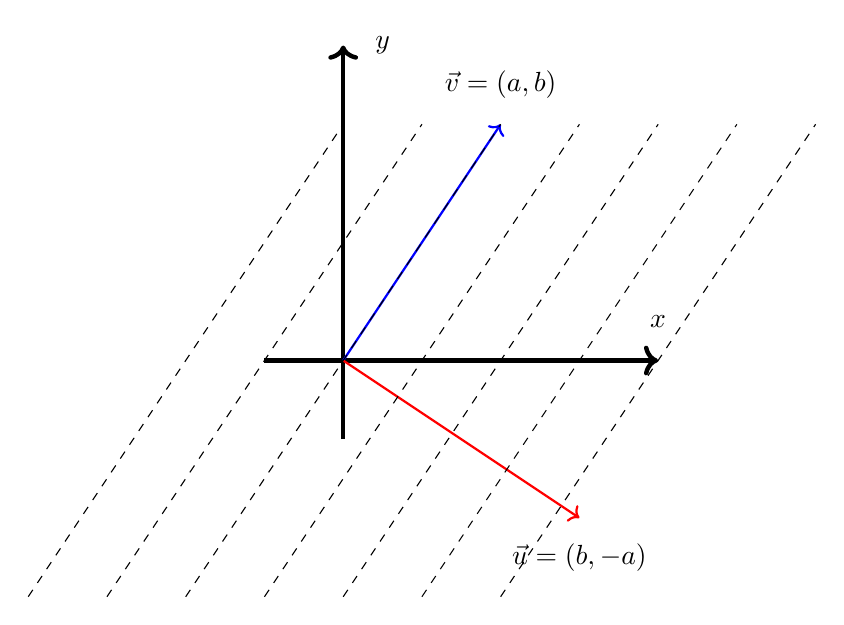
\begin{tikzpicture}
			\draw[->, ultra thick] (-1,0) -- (4,0);
			\draw[->, ultra thick] (0,-1) -- (0,4);
			\node at (4,0.5) {$x$};
			\node at (0.5,4) {$y$};
			\draw[->, color = blue, thick] (0,0) -- (2,3);
			\draw[->, color = red, thick] (0,0) -- (3,-2);
			\node at (2,3.5) {$\vec v = (a,b)$};
			\node at (3,-2.5) {$\vec u = (b,-a)$};
			\foreach {\x} in {-4,-3,-2,-1,0,1,2}
			\draw[dashed] (\x,-3) -- (\x + 4, 3);
		\end{tikzpicture}
	\end{center}
	since $u$ is constant on every one of the dashed lines. Then there exists $f : \b R \to \b R$ such that
	\[ u(x,y) = f(\vec w \cdot (x,y)) = f(bx - ay)\]
\end{proof}
\begin{proof}[Brute Force Method]
	We can simply compute
	\begin{align*}
		x' &= ax + by \\
		y' &= bx - ay \\
	\end{align*}
	then we have
	\begin{align*}
		\frac{\partial x'}{\partial x} &= a & \frac{\partial x'}{\partial y} &= b \\
		\frac{\partial y'}{\partial x} &= b & \frac{\partial y'}{\partial y} &= -b 				
	\end{align*}
	By the chain rule we have
	\begin{align*}
		u_x = \frac{\partial u}{\partial x} = \frac{\partial u}{\partial x'} \frac{\partial x'}{\partial x}	+ \frac{\partial u}{\partial y'} \frac{\partial y'}{\partial x} &= au_{x'} + bu_{y'} \\
		u_y = \frac{\partial u}{\partial y} = \frac{\partial u}{\partial x'} \frac{\partial x'}{\partial y}	+ \frac{\partial u}{\partial y'} \frac{\partial y'}{\partial y} &= bu_{x'} - au_{y'} \\
	\end{align*}
	Hence 
	\[ 0 = au_x + bu_y = a(au_{x'} + bu_{y'}) + b(bu_{x'} - au_{y'}) - (a^2 \cdot b^2)\]
	Therefore $u_{x'} = 0$, so $u(x',y') = f(y') = f(bx - ay)$, which gives us the same answer as the geometric method.
	
	
	
\end{proof}
\subsubsection{Variable Coefficient PDEs}
\begin{example}
	Find $u = u(x,y)$ such that
	\[ u_x + yu_y = 0\]
\end{example}
\begin{proof}[Solution]
	Similar to the first PDE, we can rewrite the equation as
	\[ (x,y) \cdot \nabla u = 0 \]
	\begin{center}
		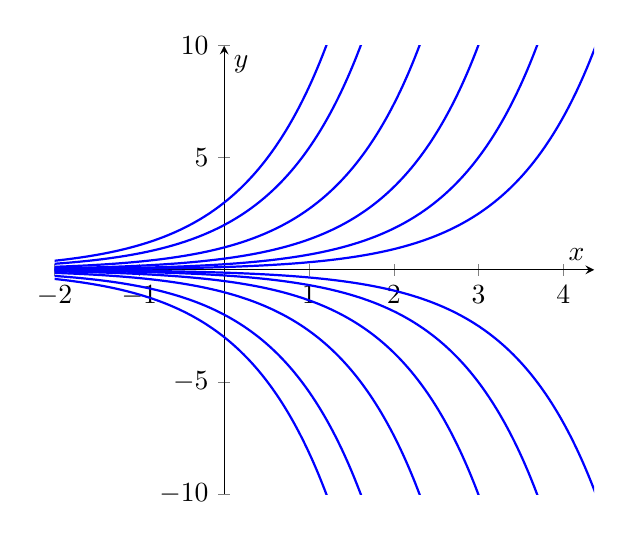
\begin{tikzpicture}
			\begin{axis}[
				samples=100,domain=-2:5, ymin = -10, ymax = 10,
				axis y line=middle,
				axis x line=middle,
				xlabel=$x$,ylabel=$y$,]
				\addplot[thick,blue,smooth] plot ({\x}, {exp(\x)});
				\addplot[thick,blue,smooth] plot ({\x}, {2*exp(\x)});
				\addplot[thick,blue,smooth] plot ({\x}, {3*exp(\x)});
				\addplot[thick,blue,smooth] plot ({\x}, {0.5*exp(\x)});
				\addplot[thick,blue,smooth] plot ({\x}, {0.25*exp(\x)});
				\addplot[thick,blue,smooth] plot ({\x}, {0.125*exp(\x)});
				\addplot[thick,blue,smooth] plot ({\x}, {-exp(\x)});
				\addplot[thick,blue,smooth] plot ({\x}, {-2*exp(\x)});
				\addplot[thick,blue,smooth] plot ({\x}, {-3*exp(\x)});
				\addplot[thick,blue,smooth] plot ({\x}, {-0.5*exp(\x)});
				\addplot[thick,blue,smooth] plot ({\x}, {-0.25*exp(\x)});
				\addplot[thick,blue,smooth] plot ({\x}, {-0.125*exp(\x)});
			\end{axis}
		\end{tikzpicture}

		The blue lines are called characteristic curves.
	\end{center}
	
	Hence consider curves with slope $y$
	\[ \frac{dy}{dx} = y.\]
	Solving for the ODE gives us
	\[ y = Ce^{x} \qquad C \in \b R.\]
	Notice that $u$ is constant on the curves.
	\[ \frac{d}{dx} \left( u \left( x, Ce^{x} \right)  \right) = u_x + u_y \cdot \frac{dy}{dx} = u_x + u_y y = 0. \]
	Hence
	\[ u(x, Ce^x) = u(0, Ce^0) = u(0,C)\]
	is independent of $x$. Now given $(x,y)$ in the place, we compute
	\[ u(x,y) = u(x,Ce^x)  =u(0,C)  = u(0, e^{-x}y)\]
	choose $C \in \b R$, we have $C = e^{-x}y \iff y = Ce^x$. Hence 
	\[ u(x,y) = f(e^{-x}y)\]
	where $f$ is a elementary function of one variable.
\end{proof}
\begin{exercise}
	Find the solution of the example above such that
	\[ u(0,y) = y^5\]
\end{exercise}
\begin{proof}[Solution]
	\[ u(0,y) = y^5 \implies u(x,y) = (e^{-x}y)^5 = y^5 e^{-5x}\]
\end{proof}
\subsection{Motivation behind PDE}
\begin{example}[Transport]
	Suppose a pipe with a pollutant suspend in the water and the water is moving along side the pipe to the right at a rate $c$, then the concentration of the pollution at time $t$ and point $x$ can be modeled as
	\[ u_t  + c u_x = 0.\]
\end{example}
\begin{example}[Vibrating String]
	Check the derivation in textbook which gives the wave equation. Suppose a string is plucked, then the displacement of the string can be modeled as
	\[ u_{tt} = c^2 u_{xx}.\]
	The three dimensional version, a vibrating drumhead can be expressed as
	\[ u_{tt} = c^2 \left( u_{xx} + u_{yy} \right) \]
\end{example}
\begin{example}[Diffusion]
	Suppose a chemical substance is diffusing through the liquid. The mass of the substance at time $t$ in any given cross section $[x_0,x_1]$ is given by
	\[ M(t) = \int_{x_0}^{x_1} u(x,t) dx\]
	We then have
	\[ \frac{dM}{dt} = \text{flow in} - \text{flow out} = ku_x(x_1,t) - ku_x(x_0,t) = \int_{x_0}^{x_1} u_t(x,t) dx.\]
	Differentiating with respect to $x$ gives
	\[u_t = k u_{xx}.\]
	In $\dim d$ we have 
	\[ \forall D \subset D_0 \qquad \int_D u_t(x,t) dx \stackrel{\text{Fluid's Law}}{=} \int_{\partial D} k(n \cdot \nabla u) \, dX \stackrel{\text{div thm}}{=} \int_{D} \mathrm{div}\,(k\nabla u)\, dx = \int_D k \triangle u\, dx\]
	By the second vanishing theorem we have
	\[ u_t - k \triangle u = 0 \qquad \mathrm{in} \quad D_0\]
\end{example}
\end{document}